\documentclass[12pt]{article}
\usepackage{polski}
\usepackage[utf8]{inputenc}
\usepackage{amsfonts}
\usepackage{amsmath}
\usepackage{enumitem}
\usepackage{graphicx}
\usepackage{float}
\usepackage{centernot}
\usepackage{mathtools}
\setlength{\parskip}{1em}


\begin{document}
	\title{Sprawozdanie\\Metody Numeryczne 2, laboratorium 6}
	\author{Grzegorz Rozdzialik (D4, grupa lab. 2)}
	\maketitle	
	
	\section{Zadanie}
	{\Large Temat \textbf{6}, zadanie \textbf{11}:}\\
	Metoda Rungego-Kutty rzędu 4-go (wzór "3/8") dla układu dwóch równań.
	
	Niech $x \in [a, b] \subset \mathbb{R}$. Dane zagadnienie początkowe do rozwiązania:
	\begin{equation}
	\begin{dcases}
		y_1' &= f_1(x, y_1, y_2) \\
		y_2' &= f_2(x, y_1, y_2) \\
		y_1(a) &= y_{1, a} \\
		y_2(a) &= y_{2, a}
	\end{dcases}
	\end{equation}
	
	Niech $n \in N$ będzie liczbą oznaczającą ilość podprzedziałów, na jakie należy podzielić odcinek $[a, b]$ tak, że:
	\begin{align*}
		h = \frac{b - a}{n} & \\
		x_0 = a & \\
		x_i = x_{i - 1} + h & \hspace{10px} \mbox{dla } i = 1, 2, \dots, n
	\end{align*}
	
	
	
	
	\section{Opis metody}
	Metoda Rungego-Kutty rzędu 4 dla pojedynczego równania różniczkowego określa się wzorem:
	\begin{equation}
		\label{eq:RK4}
		y_{n+1} = y_n + \sum_{i = 1}^{4} w_i K_i
	\end{equation}
	
	gdzie:
	\begin{align*}
		K_1 &= hf(x_n, y_n) \\
		K_i &= hf(x_n + a_i h, y_n + \sum_{j = 1}^{i - 1} b_{i, j} K_j), \hspace{10px} i > 1
	\end{align*}
	$w_i, a_i, b_{i, j}$ - stałe.
	
	Dla metody "trzech ósmych" te stałe wynoszą:
	\begin{align*}
		w = \begin{bmatrix}
			\frac{1}{8} & \frac{3}{8} & \frac{3}{8} & \frac{1}{8}
		\end{bmatrix}^T
		\\
		a = \begin{bmatrix}
			0 & \frac{1}{3} & \frac{2}{3} & 1
		\end{bmatrix}^T
		\\
		b = \begin{bmatrix}
			0 & 0 & 0 \\
			1/3 &  0  & 0 \\
			-1/3 & 1 & 0 \\
			1 & -1 &  1
		\end{bmatrix}
	\end{align*}
	
	Licząc rozwiązanie w punkcie $x_{i}, i = 1, 2, \dots, n$ należy oddzielnie obliczać wektor $K$ dla $y_1$ oraz $y_2$.
	
	
	
	\section{Implementacja metody}
	Implementacja metody podzielona jest na następujące kroki:
	\begin{enumerate}
		\item \texttt{[x, y1, y2] = solveDifferentialSystem(f1, f2, a, b, n, y1a, y2a)} - podział odcinka $[a, b]$ na $n$ podprzedziałów, wykorzystanie zagadnienia początkowego do uzupełnienia $y_{1, a}, y_{2, a}$, iteracyjne obliczenie kolejnych rozwiązań funkcją \texttt{calculateSolutionValue}
		
		\item \texttt{[y1n, y2n] = calculateSolutionValue(f1, f2, y1, y2, x, n)} - obliczenie rozwiązań $y_{1, n}$ oraz $y_{2, n}$ wykorzystując metodę Rungego Kutty rzędu 4 (wzór \eqref{eq:RK4})
		
		\item \texttt{plotResults(x, y1, y2, y1Exact, y2Exact, joinPlots)} - naniesienie wartości rozwiązania obliczonych metodą \eqref{eq:RK4} oraz wartości dokładnych na wykres. Dodatkowo utworzenie wykresu z modułem błędów dla obu metod.
	\end{enumerate}

	
	
	\section{Poprawność metody}
	Z rozdziału dotyczącego \textit{Metod Rungego-Kutty} w książce Z. Fortuna, B. Macukow, J. Wąsowski \textit{Metody numeryczne} wiadomo, że wzór "trzech ósmych" jest absolutnie stabilny dla dostatecznie małych $h$, zatem zwiększając parametr $n$, a co za tym idzie zmniejszając długość każdego z podprzedziałów (czyli zmniejszając $h$) otrzymujemy absolutną stabilność tej metody.
	
	Można to łatwo zauważyć zwiększając parametr $n$ w skrypcie testowym (opisanym w sekcji \ref{sec:testing-script}).
	
	
	
	\section{Przykłady}
	W przykładach znajdują się fragmenty konfiguracji skryptu do testowania metody (opisany w sekcji \ref{sec:testing-script}).
	
	Przykładowo, zagadnieniu początkowemu:
	\begin{align*}
	\begin{dcases}
		y_1' &= y_2 \\
		y_2' &= 3e^\frac{x}{2} - y_2 \\
		y_1(0) &= 4 \\
		y_2(0) &= 3
	\end{dcases}
	\end{align*}
	
	odpowiada następująca konfiguracja:
	\\
	\texttt{
		f1 = @(x, y1, y2)(y2); \\
		f2 = @(x, y1, y2)(3 * exp(x / 2) - y2); \\
		a = 0; \\
		b = 10; \\
		y1a = 4; \\
		y2a = 3; \\	
	}

	\begin{enumerate}[label=\textbf{Przykład \arabic*}]
		\item 
		\label{example-changingN-1}
		Zagadnienie początkowe utworzone z przekształcenia równania różniczkowego 2-go rzędu na układ równań różniczkowych 1-go rzędu.
		
		\texttt{
		f1 = @(x, y1, y2)(y2);	\\
		f2 = @(x, y1, y2)(3 * exp(x / 2) - y2);\\
		a = 0;\\
		b = 10;\\
		y1a = 4;\\
		y2a = 3;\\	
		y1Solution = @(x)(-exp(-x) + 4 * exp(x / 2) + 1); \\
		y2Solution = @(x)(exp(-x) + 2 * exp(x / 2));
		}
	
		$n = 10$
	
		\begin{figure}[H]
			\centering
			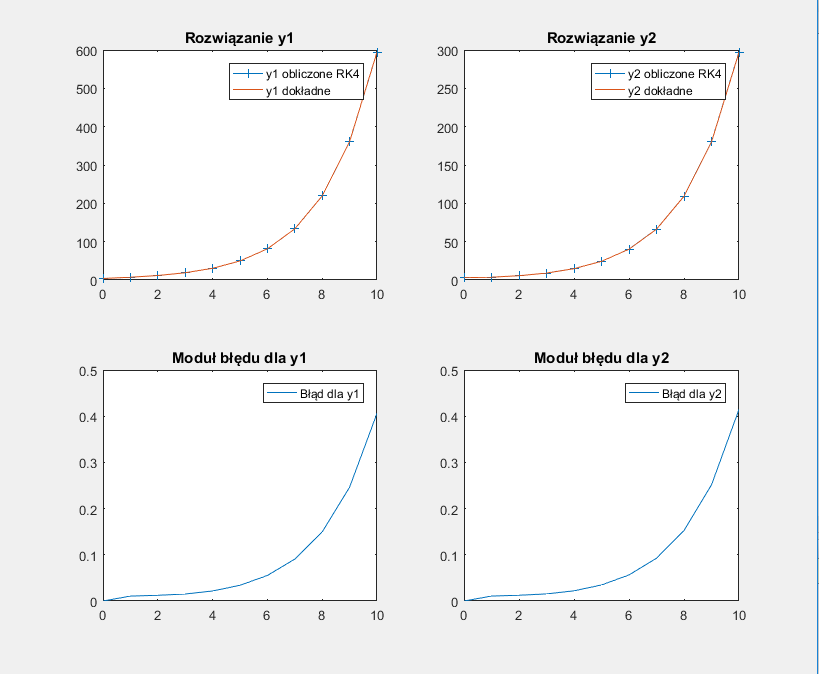
\includegraphics[scale=0.7]{images/example-1.png}
		\end{figure}
	
	
		Czas rozwiązywania zagadnienia początkowego: 0.000003 ms\\
		Maksymalny moduł błędu między rozwiązaniem dokładnym a obliczonym metodą:
		\begin{itemize}
			\item dla y1: 0.4060596
			\item dla y2: 0.4145344
		\end{itemize}
	
		Jak widać obliczenia zajmują bardzo mało czasu i są dość dokładne już dla małych wartości $n$.
		
		\item 
		\label{example-changingN-2}
		To samo zagadnienie początkowe co w poprzednim przykładzie.
		
		\texttt{
			f1 = @(x, y1, y2)(y2);	\\
			f2 = @(x, y1, y2)(3 * exp(x / 2) - y2);\\
			a = 0;\\
			b = 10;\\
			y1a = 4;\\
			y2a = 3;\\	
			y1Solution = @(x)(-exp(-x) + 4 * exp(x / 2) + 1); \\
			y2Solution = @(x)(exp(-x) + 2 * exp(x / 2));
		}
		
		10-krotnie zwiększona liczba przedziałów: $n = 100$
		
		\begin{figure}[H]
			\centering
			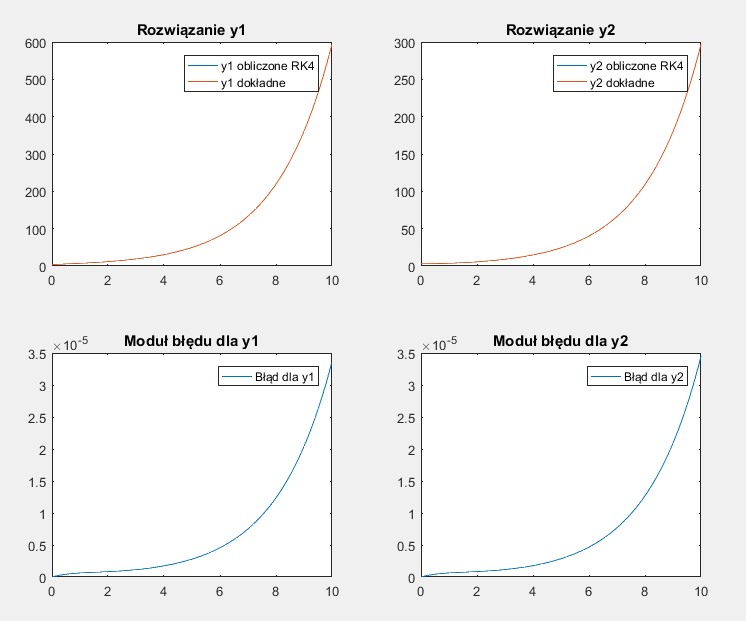
\includegraphics[scale=0.7]{images/example-2.png}
		\end{figure}
		
		
		Czas rozwiązywania zagadnienia początkowego: 0.000006 ms\\
		Maksymalny moduł błędu między rozwiązaniem dokładnym a obliczonym metodą:
		\begin{itemize}
			\item dla y1: $3.362839 * 10^{-5}$
			\item dla y2: $3.448142 * 10^{-5}$
		\end{itemize}
	
		Maksymalny błąd zmalał 10000-krotnie, a czas obliczeń wzrósł jedynie 2-krotnie.
		
		\item
		\label{example-bigN}
		
		To samo zagadnienie początkowe co w poprzednim przykładzie.
		
		10-krotnie zwiększona liczba przedziałów: $n = 1000$
		
		Wykresy wyglądają bardzo podobnie, zmienia zmienia się jedynie skala na wykresie błędów, więc nie zostały tu umieszczone, ponieważ nic nie wnoszą do przykładu.
		
		Czas rozwiązywania zagadnienia początkowego: 0.000041 ms\\
		Maksymalny moduł błędu między rozwiązaniem dokładnym a obliczonym metodą:
		\begin{itemize}
			\item dla y1: $3.274067 * 10^{-9}$
			\item dla y2: $3.359560 * 10^{-9}$
		\end{itemize}
		
		Znowu błąd zmalał 10000-krotnie. Czas obliczeń tym razem wzrósł około 7 razy.
	\end{enumerate}
	
	
	
	
	\section{Wnioski}
	\begin{enumerate}
		\item
		Na podstawie porównań maksymalnego modułu błędu można zauważyć, że metoda \eqref{eq:RK4} jest faktycznie rzędu 4, ponieważ przy 10-krotnym zwiększeniu liczby przedziałów błąd zmalał 10000-krotnie (\ref{example-changingN-1} oraz \ref{example-changingN-2}).
		
		\item
		Metoda ma złożoność O(n). Można to zauważyć zwiększając parametr $n$. Ponadto, w metodzie występuje jedynie jedna pętla zależna od ilości podprzedziałów, w której jest stała liczba obliczeń (w każdej iteracji).
		
		\item
		Metoda działa bardzo szybko nawet dla dużych $n$ ($n = 1000$ w przykładzie \ref{example-bigN}).
	\end{enumerate}
	
	
	
	\section{Skrypt do testowania metody}
	\label{sec:testing-script}
	Do testowania metody został utworzony skrypt znajdujący się w pliku \texttt{textScript.m}.
	
	Pozwala on na wpisanie własnego zagadnienia początkowego, rozwiązania tego zagadnienia (w celu obliczenia wartości dokładnych oraz wektora błędów), a także określenie ilości podprzedziałów, na jakie ma zostać podzielony odcinek $[a, b]$ (parametr $n$, zazwyczaj im większy, tym lepsza dokładność i mniejszy błąd rozwiązania).
	
	Dodatkowo można określić, czy rozwiązania mają zostać naniesione na dwóch oddzielnych wykresach, czy na jednym (parametr \texttt{joinPlots}, opis w skrypcie).
	
	
	\section{Bibliografia}
	\begin{enumerate}
		\item Informacje z wykładu \textit{Metod numerycznych 2} (wydział MiNI PW, dr Iwona Wróbel), w szczególności temat dotyczący \textit{metody Rungego-Kutty} oraz \textit{rozwiązywania układu równań różniczkowych}.
		\item Z. Fortuna, B. Macukow, J. Wąsowski \textit{Metody numeryczne} - rozdział 7 \textit{Metody rozwiązywania zagadnień początkowych dla równań różniczkowych zwyczajnych}, podrozdział 7.4 \textit{Metody typu Rungego-Kutty}.
	\end{enumerate}
	
\end{document}